\documentclass[review,12pt]{elsarticle}
\usepackage[a4paper,margin=2cm]{geometry}
\usepackage{mathptmx} % Times-compatible text and maths (pdfLaTeX has no system-font access)
\usepackage{amsmath,amssymb}
\usepackage{graphicx}
\usepackage{adjustbox}
\usepackage{booktabs}
\usepackage{xcolor}
\usepackage{tikz}
\usetikzlibrary{arrows.meta}
\usepackage{hyperref}

% Working draft. Open items are written as \todo{...} and must all be gone at submission.
\newcommand{\todo}[1]{\textcolor{red}{[TODO: #1]}}

\journal{Information Fusion}

\begin{document}

\begin{frontmatter}

\title{Efficient Communication Between a Non-Transformer Perception Agent and a Frozen Gemma Language Model: A Communication-Fidelity Benchmark of Filtered Text and a Latent Channel}

% Authorship and order to be agreed with the supervisor before submission.
\author[dmu]{Alif Tasbir}
\author[dmu]{Aboozar Taherkhani}
\affiliation[dmu]{organization={De Montfort University}, city={Leicester}, country={United Kingdom}}

\begin{abstract}
Messages between language-model agents cost time and energy, especially on edge hardware. Latent communication, which replaces text with continuous messages, has been studied only between transformers, yet sensing agents are often not transformers. We compare interfaces for such a sender. A heartbeat classifier passes events to a frozen Gemma~4 E4B model as text, including a filtered message listing only abnormal events, or through a learned linear adapter emitting four virtual tokens per event. The task, reporting the most urgent triage tier among 1 to 50 heartbeats, is a communication-fidelity benchmark: its answer is a fixed rule over the sender's outputs, so we measure what each channel costs and preserves, not clinical reasoning. Under a pre-specified analysis plan with three seeds and held-out patients, the adapter cut prompt-processing time against compact text by 24\%, 50\% and 78\% at 10, 20 and 50 events and was more accurate than calibrated text at 10 and 20 events (balanced accuracy 0.83 against 0.73). Filtered text was 0.11 to 0.17 more accurate and equally fast for single requests; under batched serving on one 12~GB GPU, the adapter's median throughput was 10 to 30\% higher and its median energy per decision 12 to 28\% lower. Event-level heart rate, interval and abnormal-run information was recoverable from the virtual tokens. The pattern largely held on a second sender and an external database. For this receiver, filtering is preferable when the question is known in advance; a latent channel suits many events carried at predictable cost.
\end{abstract}

\begin{highlights}
\item Latent channel from a non-transformer sender compared with filtered text
\item Adapter carries up to 50 events at four tokens each into a frozen model
\item Filtered text is more accurate; the adapter wins under batched serving
\item Per-slot, per-field recoverability of the virtual tokens is measured
\item A selection rule, the analysis plan and its change log are released
\end{highlights}


\begin{keyword}
agent communication \sep latent communication \sep communication efficiency \sep heterogeneous agents \sep edge inference \sep electrocardiogram
\end{keyword}

\end{frontmatter}

\section{Introduction}
\label{sec:intro}

Agents built on language models spend much of their budget talking to each other. The tokens exchanged grow with every hand-off, and much of that traffic is redundant \cite{zhang2024cut}. The cost appears as latency and energy and, on edge hardware, where memory is fixed and the longest prompt sets the batch size, as a limit on how many requests can be served at all \cite{zheng2025areview,shkolnikov2026agentmemory}. Communication efficiency is now a design problem in its own right \cite{aei2026survey}.

The literature offers three levers. The first is to \emph{say less}: prune redundant messages from the agent graph \cite{zhang2024cut}, send only the semantic packets whose expected contribution exceeds their cost \cite{dong2026bandmas}, or compress the prompt \cite{mu2023gist,ge2024icae,cheng2024xrag,jiang2023llmlingua}. The second is to \emph{reuse computation}: persist and share caches so that a receiver does not re-read what it has already read \cite{shkolnikov2026agentmemory}. The third is to \emph{send a latent message} instead of text, handing the receiver hidden states, a key--value cache or an embedding with no decoding into words. The training-free LatentMAS reports 70.8 to 83.7\% fewer tokens and 4 to 4.3 times faster inference than text on nine benchmarks \cite{zou2025latent}; cache-to-cache reports a 2.5-fold reduction in latency and 3.1 to 5.4\% higher accuracy than text \cite{fu2025cachetocache}. Other designs follow the same pattern \cite{pham2024ciphers,du2026enabling,zheng2025thought,rossi2026latentcacheflow,flamant2026bicameral,jin2026agentprimitives}, and a recent framework organises them by what is transmitted and how the receiver absorbs it \cite{liu2026beyondtokens}. Systems have begun to choose among these levers adaptively, for instance between token and cache transmission according to bandwidth \cite{dai2026tokenkv}.

All of this work assumes that the agents are language models, so that the sender's hidden state or cache is something another transformer can be trained to absorb. The agents that sense the world usually are not transformers. A wearable or bedside classifier is a convolutional or recurrent network trained for classification, and nothing about its internal vector is shaped for a language model. The one heterogeneous exception we know of connects different families of vision--language models through a shared visual channel \cite{liu2026visionwormhole}, but its senders are still language models. For a sender of this kind it is open whether a latent channel is feasible, whether it is worth building, and what it costs in inspectability.

Neighbouring work does not settle the question. Projecting a signal encoder into a language model's embedding space is established \cite{jin2024timellm,babu2025modality,zhao2025ecgchat,zhang2025sensorlm}, but those systems are built to make a language model understand a signal and are judged on accuracy. They do not treat the projection as a channel whose cost is compared with a text channel on the same task. Comparisons of latent and text communication also tend to use the text baseline that is easiest to beat. Listing every event verbatim is a poor choice when the sender can filter, which is the first lever above. Without a filtered baseline, a saving in tokens says little about whether a latent channel is worth building.

This paper compares the levers for a non-transformer sender. A small learned adapter maps the 32-dimensional context vector of a convolutional--recurrent heartbeat classifier, together with three scaled side inputs, to four virtual tokens per event in the input-embedding space of a frozen, 4-bit Gemma~4 E4B model. We compare it with three text interfaces, among them a sender-side filter, each also measured with prefix caching. The task is to report the most urgent triage tier among 1 to 50 consecutive heartbeats. Electrocardiography is the case study: deep networks already match cardiologists on it \cite{hannun2019cardiologist} and language models encode clinical knowledge \cite{singhal2023large}, so pairing a sensing agent with a reasoning agent is a natural design. The task tests \emph{communication fidelity}. The correct answer is a fixed rule applied to the sender's outputs, so a wrong answer is a failure of the channel and not of clinical knowledge. A three-line rule also solves the task, and we do not claim otherwise: the language model adds nothing to the decision here. It stands in for the general-purpose receiver of an agent system, a model shared by many senders and tasks for which no one writes a rule per task, and the benchmark isolates the channel into it. The experiment therefore measures what each interface costs and loses, under a protocol fixed before the results existed, and the results tables report the rule itself as the ceiling. We ask three questions.
\begin{itemize}
\item \textbf{RQ1 (cost).} Does the adapter reduce the tokens, time and memory of the hand-off relative to text interfaces, and under which workloads?
\item \textbf{RQ2 (accuracy).} Does it preserve the accuracy of the downstream decision?
\item \textbf{RQ3 (recoverability).} How much of each event's content can be recovered from the virtual tokens, so that the cost of opacity is measured and not asserted?
\end{itemize}

The answers do not all favour the latent channel. It keeps prompt processing flat as events are added, while text grows by about 60 tokens per event, and it is more accurate than calibrated compact text at moderate window sizes. A prompt listing only the abnormal events, the filter, is more accurate than the adapter and as fast for a single request. Its length depends on how many abnormal events a window contains, whereas the adapter's depends only on the number of events, and this decides the comparison once requests are batched. We report the result in this form because a system designer needs a rule for which lever to pull.

The contributions are as follows.
\begin{enumerate}
\item A communication-fidelity benchmark for the interface choice of a non-transformer sender, comparing the three efficiency levers (filter, reuse, latent) with a text baseline that includes a sender-side filter, on a task whose answer is fixed so that every error is the channel's.
\item A latent channel from such a sender into a frozen language model, extended from one event per call to fifty, in which the language model is untouched and only 0.88 million adapter parameters are trained.
\item A controlled evaluation of cost, accuracy and recoverability against a pre-specified analysis plan, including serving under batching and prefix caching, replication on a second sender architecture, and an external confirmatory test that confirmed both the adapter's advantage over calibrated text and the filter's advantage over the adapter (Section~\ref{sec:incart}).
\item A recoverability protocol that decodes each event's label, tier, heart rate, interval and abnormal-run status from its slot of virtual tokens, separating what the channel carries from what the receiver uses.
\item A rule for choosing between a filtered text interface and a latent one, with the analysis plan, its change log and code to reproduce every table.
\end{enumerate}

Section~\ref{sec:related} places the work among the three levers and the literature on heterogeneous senders. Section~\ref{sec:system} describes the sender, the adapter and the decoding scheme, and Section~\ref{sec:protocol} the evaluation protocol. Sections~\ref{sec:results} and~\ref{sec:discussion} report and discuss the results, with limitations.

\section{Related Work}
\label{sec:related}

We organise the related work by the three levers of communication efficiency introduced in Section~\ref{sec:intro}, then turn to the two literatures that bear on a non-transformer sender: signal encoders connected to language models, and the effects that make long text prompts fail.

\subsection{Saying Less}
The first lever reduces what is sent. AgentPrune prunes redundant messages from the spatial--temporal message-passing graph of a multi-agent system in one shot and reports 28.1 to 72.8\% fewer tokens across existing frameworks \cite{zhang2024cut}. BANDMAS splits each message into semantic packets, such as evidence and requests, and transmits only those whose predicted contribution exceeds their cost, reducing application-layer bytes by 53.2 to 77.3\% on three question-answering workloads \cite{dong2026bandmas}. Prompt-compression methods act inside the receiver's context: they train a language model to compress a prompt into a few learned tokens \cite{mu2023gist,ge2024icae}, map a retrieved document to a single token \cite{cheng2024xrag}, or prune the prompt with a small language model \cite{jiang2023llmlingua}.

These methods share an assumption: the content is text that the sender could have chosen to write more briefly. For a perception agent that reports structured events, the equivalent is a filter that lists only the events that matter and counts the rest. We construct this baseline explicitly (Section~\ref{sec:protocol}). It is the standard against which a latent channel for such a sender has to be judged, and it is absent from prior comparisons of latent and text communication.

\subsection{Reusing Computation and Choosing the Medium}
The second lever avoids recomputing what the receiver has already read. On edge devices, persisting each agent's cache in 4-bit form lets a multi-agent system resume with large reductions in time to first token \cite{shkolnikov2026agentmemory}. These measures act on the cost of reading, not on the number of tokens a message needs. We therefore report prefix caching with every arm, to check that the ranking of interfaces does not depend on it.

A growing line of work treats the medium itself as a decision. Dai et al.\ select between token and key--value-cache transmission according to system conditions and allocate wireless bandwidth jointly, reducing end-to-end latency relative to either medium used alone \cite{dai2026tokenkv}. A recent survey of communication-efficient agentic edge intelligence formalises what to send, when and to whom as a communication policy, and identifies communication as the primary design constraint at the edge \cite{aei2026survey}. Our selection rule (Section~\ref{sec:discussion}) is a policy of this kind, derived from measurements for a sender that these works do not consider.

\subsection{Latent Communication Between Language-Model Agents}
The third lever replaces the text message with a continuous one, and the designs differ in what is sent and how it is absorbed. CIPHER transmits the expectation of the vocabulary embeddings under the sender's token distribution, so that the receiver sees the sender's uncertainty as well as its sampled word \cite{pham2024ciphers}. LatentMAS shares last-layer hidden states and a latent working memory among agents without any training \cite{zou2025latent}. Cache-to-cache trains a projector and a fusion module that inject a source model's key--value cache into a target model, across model families \cite{fu2025cachetocache}. A latent cache-flow method transmits a compressed cache and equips the receiver with an adapter that translates and decompresses it \cite{rossi2026latentcacheflow}. In the bicameral model, two frozen language models are coupled through a trainable interface on their intermediate hidden states at every generation step \cite{flamant2026bicameral}. Du et al.\ train a receiver-side adapter over compressed hidden states, report up to a 24-fold speed-up from compression, and present the work as a feasibility study \cite{du2026enabling}. Thought communication exchanges latent thoughts rather than words \cite{zheng2025thought}, and reusable latent building blocks have been proposed for multi-agent pipelines \cite{jin2026agentprimitives}. Liu et al.\ organise these designs by carrier and injection mechanism \cite{liu2026beyondtokens}.

Reported benefits are lower cost and, in several cases, higher accuracy than text. What the methods share is a transformer sender. The transmitted object is a hidden state or a cache that a second transformer can be trained to absorb, and several of them require the two models to expose compatible internals or to be trained as a pair. The Vision Wormhole is the nearest heterogeneous case: it maps reasoning traces from different model families into a shared latent space through a universal codec and injects them into the receiver's visual pathway \cite{liu2026visionwormhole}. The heterogeneity is among vision--language models, and the sender is still a language model. A sender whose vector is the by-product of a classification loss on a physiological signal, with no language component, lies outside this literature.

A smaller body of work asks whether a latent channel is \emph{used}. Zhang and Emu replace the message with another example's message, with a compute-matched self-generated message or with nothing, and show that equal end-task accuracy can hide opposite mechanisms \cite{zhang2026causalaudit}. They build on the distinction between a message that depends on the sender's state and a receiver whose behaviour depends on the message \cite{lowe2019pitfalls}. Our recoverability measurements answer a different question, namely what an auditor could read back from the message, and the two are complementary (Section~\ref{sec:discussion}).

\subsection{Signal Encoders Connected to Language Models}
Connecting a non-text encoder to a language model through a learned map is established practice. Visual instruction tuning projects image features into the embedding space \cite{liu2023llava}, and Flamingo injects them through gated cross-attention \cite{alayrac2022flamingo}. For time series, Time-LLM keeps the language model frozen and reprograms input patches into its text-prototype space \cite{jin2024timellm}. Babu et al.\ apply the same idea to multichannel EEG classification with a frozen language model \cite{babu2025modality}. SensorLM aligns wearable-sensor data and language by pretraining a CLIP- and CoCa-style model on 59.7 million hours of data \cite{zhang2025sensorlm}. In electrocardiography, ECG-Chat aligns a signal encoder with a language model for dialogue \cite{zhao2025ecgchat}, ELF removes the separate encoder and lets the model read the signal directly \cite{han2026encoderfree}, and zero-shot classification combines signal and clinical-text representations \cite{liu2024zeroshot}. A benchmark of more than fifteen models for fetal monitoring found that fine-tuned language models reached the best performance in most scenarios, at a higher computational cost than domain-specific architectures \cite{wong2025llms}.

The frozen-model designs are the closest to ours in what they hold constant, but they differ in purpose. They aim to make a language model \emph{understand} a signal and are judged on the accuracy of the resulting classifier or answer. None treats the projection as a message between two agents whose cost is compared with that of a text message on the same task, none compares against a sender-filtered text interface, and none reports what can be read back from the projected tokens. Our setting adds a constraint on the other side: the perception agent is trained for classification alone, with no language-aware objective, so the adapter is the only component that learns about the language model.

\subsection{Why Long Text Prompts Degrade}
Two documented effects explain why a text baseline weakens as events are added. Language models use information in the middle of a long context less well than information at its start or end \cite{liu2024lost}, and the bias can be partly corrected by calibrating positional attention \cite{hsieh2024found}. Separately, few-shot predictions are biased toward certain labels, which a calibration of the output scores corrects \cite{zhao2021calibrate}. We find the label bias clearly in our text arms and weak, inconclusive evidence of a position effect (Section~\ref{sec:results}); following the first, we report text with a calibrated routine bias as the fair comparison instead of the default prompt.

\subsection{Gap}
Saying less, reusing computation and sending latent messages have each been studied for agents that are language models. What has not been shown is a controlled, same-task comparison of these levers for a \emph{non-transformer sender}, in which the text baseline \emph{includes a sender-side filter}, the receiver is frozen throughout, cost is measured under serving conditions, and the information a latent channel preserves is measured and not assumed. The remainder of the paper supplies that comparison.

\section{System}
\label{sec:system}

Figure~\ref{fig:pipeline} shows the pipeline. A perception agent classifies each heartbeat and emits an event. The events of a window cross an interface to a reasoning agent, which returns a structured triage decision. Only the interface varies between arms, and each arm implements one of the efficiency levers of Section~\ref{sec:intro} (Table~\ref{tab:levers}), so the comparison is one of levers on a fixed sender and a fixed receiver.

\begin{table}[t]
\caption{The interfaces compared, and the efficiency lever each implements. Prefix caching is applied to every arm as a second condition and is not a separate arm.}
\label{tab:levers}
\centering
\small
\begin{tabular}{lll}
\toprule
Arm & Lever & What crosses the interface \\
\midrule
A-full & none (reference) & Full record of every event, as text \\
A-compact & none (baseline) & One compact line per event, as text \\
A-filtered & say less & Abnormal events only, normal events as a count \\
Adapter (r4) & send latent & Four virtual tokens per event \\
\bottomrule
\end{tabular}
\end{table}

\begin{figure}[t]
\centering
\adjustbox{max width=\linewidth}{% Figure 1: system overview, included from sections/system.tex.
% Palette matches the data figures: orange = text with every event, violet = filtered text, blue = latent adapter.
% Grey fill = frozen component; thick coloured border + "TRAINED" badge = the one trained part.
\definecolor{cA}{HTML}{EB6834}
\definecolor{cF}{HTML}{4A3AA7}
\definecolor{cL}{HTML}{2A78D6}
\definecolor{cX}{HTML}{C0392B}
{\renewcommand{\baselinestretch}{1}\selectfont
\begin{tikzpicture}[font=\normalsize,
  frozen/.style={draw=black!55, rounded corners=3pt, align=center, inner sep=6pt, fill=black!6, text width=#1},
  lane/.style={draw=#1, line width=1pt, rounded corners=4pt, fill=#1!6, inner sep=0pt},
  tok/.style={draw=#1!80!black, fill=#1!35, minimum width=2.1mm, minimum height=4.2mm, inner sep=0pt, line width=0.4pt},
  arr/.style={-{Stealth[length=2.4mm]}, line width=0.9pt, black!60},
  lab/.style={font=\small, text=black!75, align=center, inner sep=1.5pt},
  badge/.style={font=\scriptsize\bfseries, text=white, fill=cL, rounded corners=2pt, inner sep=2.5pt}]

% ---- ECG strip with beat labels ------------------------------------------------------------------------
\def\qrs#1#2{\draw[line width=1pt,#2] (#1-0.45,0)--(#1-0.2,0)--(#1-0.1,0.18)--(#1,1.1)--(#1+0.12,-0.4)--(#1+0.24,0)--(#1+0.55,0);}
\node[font=\small\bfseries, anchor=south west] at (-0.2,1.9) {1. Sense};
\draw[black!35, line width=0.5pt] (-0.2,0)--(5.4,0);
\qrs{0.5}{black!80} \qrs{1.6}{black!80} \qrs{2.7}{cX} \qrs{3.8}{black!80} \qrs{4.9}{cX}
\foreach \x/\t/\c in {0.5/N/black!70,1.6/N/black!70,2.7/V/cX,3.8/N/black!70,4.9/S/cX}{\node[font=\small\bfseries,text=\c] at (\x,-0.75) {\t};}
\node[lab, anchor=north] at (2.6,-1.25) {$N$ consecutive heartbeats\\(here $N=5$)};

% ---- perception agent and events -------------------------------------------------------------------------
\node[font=\small\bfseries, anchor=south west] at (6.4,1.9) {2. Classify (frozen)};
\node[frozen=38mm] (per) at (8.3,0) {\textbf{Perception agent}\\CNN--LSTM + RR branch\\\emph{not a transformer}};
\draw[arr] (5.55,0)--(per.west);

\node[font=\small\bfseries, anchor=south west] at (11.9,1.9) {3. Report $N$ events};
\node[frozen=40mm] (ev) at (14.0,0) {context vector $\mathbf{z}_i\in\mathbb{R}^{32}$\\[1pt]label, confidence,\\heart rate, RR, run length};
\draw[arr] (per.east)--(ev.west);

% ---- three interfaces -------------------------------------------------------------------------------------
\node[font=\small\bfseries, anchor=south west] at (17.9,5.6) {4. Cross one of three interfaces};

% lane A: text, every event
\node[lane=cA, minimum width=74mm, minimum height=21mm] (la) at (22.0,3.6) {};
\node[font=\small\bfseries, text=cA!70!black, anchor=north west] at (18.3,4.6) {A-compact (baseline)};
\foreach \i in {0,...,17}{\node[tok=cA] at (18.65+0.27*\i,3.55) {};}
\node[lab, anchor=west] at (23.55,3.55) {$\ldots$};
\node[lab, anchor=north west] at (18.3,3.05) {every event as text: $\approx$60 tokens per event};

% lane B: filtered text
\node[lane=cF, minimum width=74mm, minimum height=21mm] (lb) at (22.0,0) {};
\node[font=\small\bfseries, text=cF!80!black, anchor=north west] at (18.3,1.0) {A-filtered (lever: say less)};
\foreach \i in {0,...,5}{\node[tok=cF] at (18.65+0.27*\i,-0.05) {};}
\node[lab, anchor=west, text=cX] at (20.35,-0.05) {V};
\foreach \i in {0,...,5}{\node[tok=cF] at (20.9+0.27*\i,-0.05) {};}
\node[lab, anchor=west, text=cX] at (22.65,-0.05) {S};
\node[draw=cF!80!black, fill=white, font=\scriptsize, inner sep=2pt, rounded corners=1pt] at (24.1,-0.05) {3 normal};
\node[lab, anchor=north west] at (18.3,-0.55) {abnormal events as text, normals as a count};

% lane C: latent adapter
\node[lane=cL, line width=2pt, minimum width=74mm, minimum height=21mm] (lc) at (22.0,-3.6) {};
\node[font=\small\bfseries, text=cL!80!black, anchor=north west] at (18.3,-2.6) {Adapter (lever: send latent)};
\node[badge, anchor=north east] at (25.5,-2.58) {TRAINED};
\foreach \g in {0,...,4}{\foreach \i in {0,...,3}{\node[tok=cL] at (18.65+1.3*\g+0.26*\i,-3.65) {};}}
\node[lab, anchor=north west] at (18.3,-4.15) {every event as 4 virtual tokens: $\mathbf{W}[\mathbf{z}_i;\mathbf{s}_i]+\mathbf{P}_i$};

\draw[arr] (ev.east)--++(0.9,0) |- (la.west);
\draw[arr] (ev.east)--(lb.west |- ev.east);
\draw[arr] (ev.east)--++(0.9,0) |- (lc.west);

% ---- reasoning agent -------------------------------------------------------------------------------------
\node[font=\small\bfseries, anchor=south west] at (26.9,5.6) {5. Decide (frozen)};
\node[frozen=36mm, minimum height=118mm] (llm) at (29.3,0) {\textbf{Reasoning agent}\\Gemma 4 E4B\\frozen, 4-bit\\[6pt]scaffold +\\schema-constrained\\decoding\\[8pt]$\downarrow$\\[2pt]\texttt{\{"tier": "urgent",}\\\texttt{ "beat": 3\}}};
\draw[arr] (la.east)--(llm.west |- la.east);
\draw[arr] (lb.east)--(llm.west |- lb.east);
\draw[arr] (lc.east)--(llm.west |- lc.east);

% ---- legend ----------------------------------------------------------------------------------------------
\node[frozen=0mm, minimum width=5mm, minimum height=4mm, inner sep=0pt] at (18.3,-6.2) {};
\node[lab, anchor=west] at (18.75,-6.2) {frozen (never updated)};
\node[draw=cL, line width=2pt, minimum width=5mm, minimum height=4mm, inner sep=0pt, fill=cL!6] at (22.4,-6.2) {};
\node[lab, anchor=west] at (22.85,-6.2) {the only trained part};
\node[draw=black!60, fill=black!25, minimum width=2.1mm, minimum height=4.2mm, inner sep=0pt, line width=0.4pt] at (26.4,-6.2) {};
\node[lab, anchor=west] at (26.75,-6.2) {= one token};
\end{tikzpicture}}
}
\caption{System overview. A perception agent that is not a transformer classifies each heartbeat, and the events of a window (abnormal beats in red) cross one of three interfaces to a frozen reasoning agent. Each small square is one token: text grows with every event (about 60 tokens each), the filter lists only abnormal events and counts the rest, and the adapter sends four virtual tokens per event. Grey boxes are frozen; only the adapter (blue) is trained. Sender, receiver and decoding are identical across arms, and the message sizes are the measured medians of Section~\ref{sec:results}.}
\label{fig:pipeline}
\end{figure}

\subsection{Task}
Each window contains $N$ consecutive heartbeats from one recording, with $N \in \{1,5,10,20,50\}$. The reasoning agent must return the most urgent triage tier in the window and say which beat set it. The tier of a single beat follows a fixed escalation rule applied to the perception agent's event: \emph{urgent} if the event requires urgent review (a run of three or more consecutive abnormal beats, or a single ventricular or fusion beat classified with confidence of at least 0.85), \emph{routine} if the beat is classified as normal, and \emph{priority} otherwise. The reference tier of a window is the maximum over its beats. The rule is applied to the perception agent's \emph{predictions}, not to the annotations, because the test is whether the channel delivers the sender's output faithfully; agreement with the annotations is reported separately (Section~\ref{sec:results}). The task is a communication-fidelity benchmark, not a clinical reasoning task. A fixed rule over the perception outputs solves it, so it cannot show that a language model adds clinical judgement.

\subsection{Perception Agent}
The perception agent is a convolutional--recurrent classifier trained only on the five-class AAMI EC57 beat task \cite{aami1998ec57}. A 360-sample window (1~s at 360~Hz) passes through three one-dimensional convolutional blocks (32, 64 and 128 channels, with batch normalisation, ReLU and max-pooling), a bidirectional LSTM with hidden size 64, and a unidirectional context LSTM with hidden size 32. The output of the context LSTM, a 32-dimensional \emph{context vector}, feeds the classification head and is the only representation passed downstream. There is no pretraining, no contrastive objective and no auxiliary loss.

The original design saw a single window and no timing, yet the text interface carried the RR interval, so a five-feature RR branch (previous and next RR interval, local mean RR and two ratios) was added to the context stage. Across ten training seeds it improved overall accuracy from 0.854 to $0.926 \pm 0.019$, ventricular sensitivity from 77\% to $93\% \pm 3\%$ and the class recoverability of the context vector from 69.6\% to $81.2\% \pm 5.0\%$, at the cost of one beat of latency. Fusion-beat detection stayed poor ($5\% \pm 7\%$ sensitivity). All adapters were trained on seed~0 of this encoder, which ranked third, fourth and seventh of ten on accuracy, supraventricular sensitivity and recoverability and was designated representative by a rule fixed beforehand.

A second, purely convolutional sender (residual one-dimensional convolutions without recurrence, the same RR branch and the same 32-dimensional vector) tests whether the channel depends on the first sender's architecture (Section~\ref{sec:results}).

\subsection{Reasoning Agent}
The reasoning agent is Gemma~4 E4B, loaded in 4-bit NF4 quantisation and frozen in every arm; neither adapter training nor calibration updates its weights. The model uses per-layer embeddings, a lookup keyed by token identity, which virtual tokens lack, so virtual positions receive the lookup of a padding token. This is an architectural cost of the latent channel and applies to every adapter result.

\subsection{Adapter: the Latent Channel}
The adapter is the third lever. Its single-event form, one linear layer from the 32-dimensional vector to four tokens with 337,920 trainable parameters, was described in the first author's MSc dissertation \cite{tasbir2026dissertation}. Here it is extended to many events and retrained, with the position embeddings, normalisation and side inputs described below. The setting imposes three requirements: the sender is unchanged and is not a transformer, the receiver is unchanged, and the message length depends only on the number of events. A linear map from the sender's own vector meets all three and keeps each event's tokens a function of that event alone. For event $i$ with context vector $\mathbf{z}_i \in \mathbb{R}^{32}$ and three scaled side inputs $\mathbf{s}_i \in \mathbb{R}^{3}$ (heart rate, RR interval and abnormal-run length, each clipped and standardised), the adapter forms $\mathbf{x}_i = [\mathbf{z}_i; \mathbf{s}_i] \in \mathbb{R}^{35}$ and produces $k=4$ virtual tokens
\begin{equation}
\mathbf{T}_i = \gamma \cdot \mathrm{norm}\!\left(\mathbf{W}\mathbf{x}_i + \mathbf{b} + \mathbf{P}_i\right) \in \mathbb{R}^{4 \times 2560},
\end{equation}
where $\mathbf{W}$ and $\mathbf{b}$ define one linear map from 35 to $4 \times 2560$ dimensions, $\mathbf{P}_i \in \mathbb{R}^{4\times 2560}$ is a learned embedding for event position $i$ (up to 50 positions), $\mathrm{norm}$ rescales each token to unit length, and $\gamma$ is one learnable scalar initialised to the median norm of the embeddings the model computes for real tokens. Without the normalisation the norm of the virtual tokens drifted far from that of real tokens, and many of them together broke generation. The window's tokens are the $\mathbf{T}_i$ concatenated in event order, in place of the events' text, so prompt length depends only on $N$.

Because the map is linear and acts on one event at a time, slot $i$ is a function of event $i$ alone, so each event's content can be audited independently (Section~\ref{sec:results}). The map has rank at most 35, so the adapter cannot introduce information absent from its input. The adapter has 880,641 trainable parameters (358,400 in the projection weights, 10,240 in its bias, 512,000 in the position embeddings and one scale), against the roughly four billion effective parameters of the frozen model.

Each window's training target is a JSON answer in the interface schema (the urgency tier, a templated justification and a guideline fact), built deterministically from the reference tier. Training uses teacher forcing: the correct answer's tokens follow the virtual tokens, and the loss is token-level cross-entropy over the answer only, $L = 4\,L_{\mathrm{tier}} + L_{\mathrm{rest}}$, where $L_{\mathrm{tier}}$ averages over the tokens that spell the tier and $L_{\mathrm{rest}}$ over the other target tokens. Gradients pass through the frozen language model to the adapter, and only the adapter's parameters are updated. We used AdamW at a learning rate of $5\times10^{-4}$, warm-up over the first 5\% of steps and cosine decay to 10\% of the peak, gradient clipping at 1.0, a batch of one window and at most three epochs, with validation every quarter epoch, early stopping from the second epoch, and the checkpoint with the best validation balanced accuracy. Recipe r4 trains on 447 windows spread over $N$ from 1 to 50 and validates on 170 windows from three held-out recordings. Figure~\ref{fig:training} shows the flow.

\begin{figure}[t]
\centering
\adjustbox{max width=\linewidth}{% Figure 2: how the adapter is trained, included from sections/system.tex.
% Grey fill = frozen; blue with thick border = trained; red = loss and the backward path (dashed).
\definecolor{cL}{HTML}{2A78D6}
\definecolor{cX}{HTML}{C0392B}
{\renewcommand{\baselinestretch}{1}\selectfont
\begin{tikzpicture}[font=\normalsize,
  frozen/.style={draw=black!55, rounded corners=3pt, align=center, inner sep=6pt, fill=black!6, text width=#1},
  io/.style={draw=black!40, rounded corners=3pt, align=center, inner sep=6pt, fill=white, text width=#1},
  train/.style={draw=cL, line width=2pt, rounded corners=3pt, align=center, inner sep=6pt, fill=cL!8, text width=#1},
  loss/.style={draw=cX, line width=1pt, rounded corners=3pt, align=center, inner sep=6pt, fill=cX!7, text width=#1},
  arr/.style={-{Stealth[length=2.4mm]}, line width=0.9pt, black!60},
  back/.style={-{Stealth[length=2.4mm]}, line width=1.1pt, dashed, cX!80},
  tok/.style={draw=cL!80!black, fill=cL!35, minimum width=2.1mm, minimum height=4.2mm, inner sep=0pt, line width=0.4pt},
  lab/.style={font=\small, text=black!75, align=center, inner sep=1.5pt}]

\node[io=40mm] (win) at (0,0) {\textbf{Training window}\\$N$ events, $N$ from 1 to 50,\\incl.\ hard-negative routine windows};
\node[frozen=40mm] (per) at (6.8,0) {\textbf{Perception agent}\\frozen\\gives $\mathbf{z}_i\in\mathbb{R}^{32}$ and side inputs $\mathbf{s}_i$};
\draw[arr] (win)--(per);

\node[train=60mm] (ad) at (14.6,0) {\textbf{Adapter}\\$\mathbf{T}_i=\gamma\,\mathrm{norm}(\mathbf{W}[\mathbf{z}_i;\mathbf{s}_i]+\mathbf{b}+\mathbf{P}_i)$\\880{,}641 trainable parameters};
\draw[arr] (per)--(ad);

\node[frozen=46mm, minimum height=26mm] (llm) at (24.0,0) {\textbf{Reasoning agent (frozen)}\\input: scaffold text, virtual tokens,\\then the correct answer tokens\\\emph{(teacher forcing)}};
\draw[arr] (ad.east)--(llm.west);
\foreach \i in {0,...,7}{\node[tok] at (18.85+0.27*\i,0.55) {};}
\node[lab, anchor=north] at (19.7,-0.05) {$4N$ virtual\\tokens};

\node[io=46mm] (tgt) at (24.0,5.4) {\textbf{Target answer}\\JSON: tier, templated justification,\\guideline fact\\(built from the reference tier)};
\draw[arr] (tgt)--(llm);

\node[loss=46mm] (ls) at (24.0,-5.0) {\textbf{Loss}\\$L = 4\,L_{\mathrm{tier}} + L_{\mathrm{rest}}$\\cross-entropy over the answer tokens only};
\draw[arr] (llm)--(ls);

\draw[back] (ls.west)--(ad.south |- ls.west)--(ad.south);
\node[lab, text=cX!80!black, anchor=south west] at (14.9,-4.6) {gradients pass through the frozen model;\\only the adapter is updated};

\node[io=44mm] (sel) at (6.8,-5.0) {\textbf{Schedule and selection}\\AdamW, lr $5\times10^{-4}$, batch of one;\\validation every quarter epoch,\\best balanced accuracy kept};
\end{tikzpicture}}
}
\caption{How the adapter is trained. The frozen perception agent supplies each event's vector and side inputs, the adapter (blue, the only trained part) turns them into virtual tokens, and the frozen reasoning agent is run on the scaffold, the virtual tokens and the correct answer (teacher forcing). The loss weights the tier tokens four times as heavily as the rest. Gradients (dashed) flow back through the frozen model but update only the adapter.}
\label{fig:training}
\end{figure} The final recipe, r4, differs from the earlier recipe r3 in two ways, both pre-registered before training. First, 72 training and 23 validation windows were added in which a normal beat is classified with confidence below 0.8 (\emph{hard negatives}), because r3 raised false alarms on exactly such windows. Second, the three side inputs were added, because heart rate, interval and run length were present in the text interface but could not be recovered from the 32-dimensional vector. The two changes were made together, and an ablation separates their effects (Section~\ref{sec:results}).

\subsection{Text Interfaces}
All text arms use the same scaffold, instructions and decoder as the adapter arm. They differ only in how the events are written into the prompt. A-compact and A-full list every event and so involve no effort to say less; A-filtered is the sender-side filter, the first lever.
\begin{itemize}
\item \textbf{A-compact:} one line per event with class, confidence, run length and signal quality. This is the strongest text arm that lists every event and is the primary comparator.
\item \textbf{A-full:} the full JSON record of each event, as in the earlier single-event study, reported only for cost.
\item \textbf{A-filtered:} only the non-normal events, with their position in the window, and the number of normal events as a count. No task information is lost: the filtered window yields the reference tier on all 1,195 test windows.
\end{itemize}
A text arm that lists every event is also reported under a \emph{calibrated} threshold (Section~\ref{sec:protocol}).

\subsection{Schema-Constrained Decoding}
Free generation produced malformed JSON in 9 to 20\% of answers across arms, through misnamed fields and loops. Every arm therefore uses the same constrained decoder. The structure of the answer is forced, the tier is restricted to the three valid words and chosen by the model's own scores, and free-text fields cannot close or break the structure. Every arm then produces a valid answer on every window. A check of 380 windows confirmed that the decoder changes no tier.

\section{Evaluation Protocol}
\label{sec:protocol}

The protocol is designed so that a difference between arms can be attributed to the lever, not to the prompt, the model or the measurement. It fixes the sender, receiver, scaffold and decoder, measures cost on the prompt side and under serving conditions, and scores accuracy with a rule agreed before the results existed.

\subsection{Analysis Plan and Change Log}
The study was not recorded in a third-party study registry. Instead, the analysis plan, with its endpoints, comparators, statistics and decision rules, was committed to version control on 22 September 2026, before any run of the extended study. Every later change of design went into a numbered log, with its date and reason, before the data it affected existed; earlier text was never edited. Analyses run after seeing results are labelled exploratory. The change log has 29 numbered entries, some with lettered amendments; the last, a training-data scaling curve, was stopped before it produced any result. For the external test the order is stricter: the confirmatory plan was committed before the external database was downloaded, the system was then frozen by a manifest of file hashes and a release tag, and the hash of the test-window list was committed before any model output on that database existed. Commit timestamps are self-declared, so we release the complete version history, including the change log, the freeze manifest and every result file, in an archived snapshot, so that the order of plan, data and results can be checked commit by commit. We describe this as a time-stamped analysis plan held in version control. We say where a change of design altered an outcome, and where a rule fixed in advance gave an answer we do not read literally (Section~\ref{sec:results}).

\subsection{Data}
\textbf{Training and primary test.} The MIT-BIH Arrhythmia Database \cite{moody2001impact} was used with the inter-patient split of de~Chazal et al.\ \cite{dechazal2004automatic}: 22 records for training and 22 for testing, with no patient in both, after the four paced records were excluded. Of the training records, 19 were used for training and three held out entirely for validation, so that no tuning decision touched a test patient. Beats were extracted as 360-sample windows centred on the annotated R peak and standardised per window, and annotations were mapped to the five AAMI classes. The test set contains no unclassifiable beats, a property of the split.

\textbf{Chronological replay.} The abnormal-run count is state carried across beats of a record. Events were therefore produced by replaying each record in order from its start through the frozen perception agent, so that the run count and RR interval of every window are those a deployed system would have computed.

\textbf{Test windows.} A fixed sampler (seed 0) draws windows from the test records, stratified by reference tier and by the class of the window's most urgent beat, at most three per record per cell, so that urgent and priority windows are not dominated by one class. The primary set has 1,195 windows from 22 patients, of which 400 are drawn at natural prevalence to measure false alarms. Cells that cannot be filled are left short and the achieved counts are reported in Table~\ref{tab:windows}.

\begin{table}[t]
\caption{Test windows by number of events per prompt $N$ and reference tier (primary DS2 set, 22 records). Stratified windows are drawn per tier; natural-prevalence windows are drawn without stratification and measure false alarms at real tier frequencies. Cells shorter than their quota (for example priority at $N=50$) are those the test records could not fill.}
\label{tab:windows}
\centering
\footnotesize
\adjustbox{max width=\linewidth}{\begin{tabular}{rrrrrrr}
\toprule
$N$ & Routine & Priority & Urgent & Stratified & Natural prevalence & Total \\
\midrule
1 & 60 & 60 & 57 & 177 & --- & 177 \\
5 & 60 & 59 & 56 & 175 & 100 & 275 \\
10 & 60 & 53 & 56 & 169 & 100 & 269 \\
20 & 57 & 45 & 55 & 157 & 100 & 257 \\
50 & 40 & 37 & 40 & 117 & 100 & 217 \\
All &  &  &  & 795 & 400 & 1195 \\
\bottomrule
\end{tabular}
}
\end{table}

\textbf{External confirmatory data.} The St Petersburg INCART 12-lead arrhythmia database \cite{goldberger2000physionet} (75 half-hour recordings from 32 patients) was fixed as the confirmatory test before it was downloaded or inspected. Lead II is resampled from 257 to 360~Hz and converted with the same procedure, and no INCART data are used for training, tuning or prompt design. The adapter, the text prompts and the calibration biases are frozen and hashed in a manifest before the run. The results are reported in Section~\ref{sec:incart}.

\subsection{Comparators and Calibration}
The comparators are A-compact, A-full (cost only) and A-filtered (Table~\ref{tab:levers}). Reusing computation, the second lever, is not an arm: prefix caching is switched on and off for every arm in the serving measurements, to check the ranking of the other levers under it. A text model with every event listed is biased toward answering ``routine'' on long prompts, an effect known from few-shot prompting \cite{zhao2021calibrate}. To avoid a strawman we report each text arm under default decoding and with a bias added to the routine score at the tier step, chosen on the held-out validation windows only and then frozen. The calibrated arm is the fair comparison and is used for every inferential statement.

\subsection{Endpoints and Statistics}
\textbf{Accuracy.} The primary endpoint is balanced accuracy, the mean recall over the tiers present, so that the rare urgent tier carries the same weight as the common routine tier. Arms are compared on the same windows (paired). Because windows from one patient are correlated, confidence intervals use a patient-cluster bootstrap with 20,000 resamples and percentile 95\% limits. The primary question for the adapter against calibrated text is non-inferiority with a margin of $-0.05$, tested first, followed by superiority where non-inferiority holds, in a fixed order at $\alpha = 0.05$. Adapter results are the mean of three training seeds, and seed ranges are reported.

\textbf{False alarms.} The share of routine windows at natural prevalence that the arm escalates to priority or urgent.

\textbf{Cost.} Token counts of the prompt; time to first token (prompt processing) and time to the tier token (the decision), at batch size one with arm order rotated; context memory; and GPU energy. We report time to the decision, not time to the full answer, because answer length differs across arms while decode speed is identical (about 160~ms per token); the full answer would credit the interface with differences in the length of the justification. Cost medians use a paired bootstrap of the relative difference on 21 windows per $N$.

\textbf{Serving.} Throughput and energy per decision were measured with batches of one, four and eight, repeated three times, and with prefix caching on and off. The framework was capped at 90\% of the card's memory so that a batch that does not fit is recorded as such instead of being silently paged into system memory, which would measure paging and not the model. Energy is the GPU board power reported by the NVIDIA Management Library, sampled at 100~Hz in a background thread during each timed generation call (prompt processing and generation up to the tier token) and integrated over the call's wall-clock time with the trapezoid rule; energy per decision is the batch's energy divided by the batch size. The measurement covers the whole board, including its idle and static draw, and excludes the processor, host memory and the rest of the system; every call spanned at least 87 power samples. Each configuration was measured on every window chunk in each of the three repeats (63 measurements per cell at batch one, 15 at batch four and 6 at batch eight), and we report the median with the interquartile range. Serving was measured for one adapter (the first training seed), so the spread reflects measurement and content variation, not training variation.

\textbf{Recoverability.} For each event, a decoder is trained on the training records to predict label, tier, heart rate, RR interval and abnormal-run status from the virtual tokens of a given slot, and tested on the test records. The same decoder family is trained on the 32-dimensional input and on the 35-dimensional input including side inputs, so that the loss attributable to the channel is the gap between the two. Decoders are fitted per slot (slots 0, 9, 19 and 49). The decoder fixed in advance is a small multilayer perceptron; a linear decoder is fitted alongside it for comparison. Run status is scored as balanced accuracy for a run of three or more beats, because $R^2$ is ill-posed for the heavy-tailed run length on this split (a change recorded before any data from it were analysed).

\subsection{Implementation and Reproducibility}
All experiments ran on one workstation with an NVIDIA RTX 5070 (12~GB), Python 3.13 and HuggingFace \texttt{transformers} with \texttt{bitsandbytes}. Production serving engines do not accept continuous input embeddings, so absolute latencies are higher than an optimised engine would give; every arm shares this, so only relative comparisons are meaningful. Every run records its git commit, checkpoint hashes, seed and library versions. Adapter training checkpoints resume bit-identically, and one run was paused and resumed without effect on the result. The tables and figures are generated from the result files by scripts in the supplementary release. \todo{Add repository and archive DOI after the freeze.}

\section{Results}
\label{sec:results}

All numbers in this section come from the evaluation on the MIT-BIH test set (DS2) fixed in the analysis plan (1,195 windows, 22 patients) unless stated otherwise, and the tables and figures are generated from the result files by the scripts in the supplementary release. Adapter values are means of three training seeds. Intervals are 95\% patient-cluster bootstrap limits.

The subsections answer the three research questions in turn: what the latent lever costs relative to the others (RQ1), what it gives up or gains in the decision (RQ2), and what can still be read back from the message (RQ3). Each comparison is against the strongest text arm available for the question: calibrated compact text for accuracy against listing every event, and filtered text for any claim that the latent channel is worth building. Section~\ref{sec:discussion} combines the three answers into a selection rule.

\subsection{RQ1: Cost of the Interface}
At a single event the adapter has nothing to save. Its four tokens replace about 57 tokens of compact text, but the fixed scaffold dominates the prompt (end-to-end lengths of 486 and 458 tokens for the two arms in the single-event study), and time to first token is unchanged. The advantage appears only when a prompt carries many events (Table~\ref{tab:cost}). Text grows by about 60 tokens per event whereas the adapter adds four, so the adapter's prompt-processing time stays near 183~ms from 1 to 50 events while the time of compact text rises to 845~ms. Time to the tier token falls less because the decision includes generating the first answer tokens, which costs the same in both arms.

\begin{table}[t]
\caption{Cost of the adapter relative to compact text (batch one, median over 21 windows per $N$).}
\label{tab:cost}
\centering
\small
\adjustbox{max width=\linewidth}{\begin{tabular}{rrrrrr}
\toprule
$N$ & Tokens (text / adapter) & TTFT ms (text / adapter) & TTFT & Decision & Context MB \\
\midrule
1 & 576 / 516 & 181 / 184 & 0\% & $+1\%$ & --- \\
5 & 811 / 532 & 197 / 182 & $-8\%$ & $-1\%$ & $-$36 \\
10 & 1105 / 553 & 241 / 183 & $-24\%$ & $-4\%$ & $-$79 \\
20 & 1694 / 593 & 360 / 181 & $-50\%$ & $-14\%$ & $-$177 \\
50 & 3457 / 713 & 845 / 183 & $-78\%$ & $-36\%$ & $-$460 \\
\bottomrule
\end{tabular}
}
\end{table}

\begin{figure}[t]
\centering
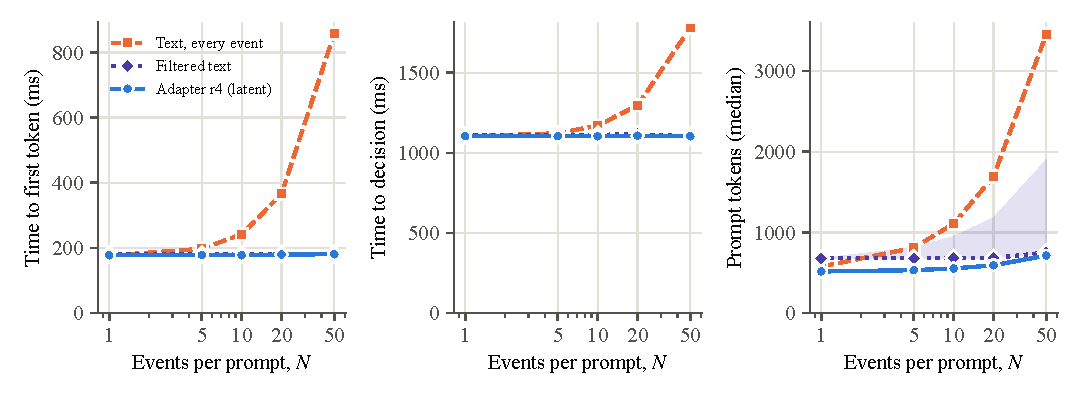
\includegraphics[width=\linewidth]{figures/fig_cost.pdf}
\caption{Cost of the three interfaces against the number of events per prompt (batch one, median of 21 windows per $N$). The shaded band in the right panel is the 90th percentile of the filtered prompt: its length depends on content, whereas the adapter's depends only on $N$. Time to decision is almost identical for filtered text and the adapter.}
\label{fig:cost}
\end{figure}

\textbf{Serving.} Single-request timing flatters neither arm because nothing is reused. Under batching, text that lists every event could not be served at a batch of eight at any $N \ge 10$, nor at a batch of four at 50 events, on the 12~GB card, whereas the adapter fitted every configuration with a peak of about 10~GB. Against A-filtered, the adapter was within about 5\% in time and throughput for single requests, with 3 to 12\% less energy per decision and overlapping interquartile ranges. Once requests were batched, its median throughput was 10 to 30\% higher and its median energy per decision 12 to 28\% lower (Table~\ref{tab:serving}), but at a batch of four the interquartile ranges of the two arms overlap for throughput at 10 and 50 events and for energy at 50 events, because the cost of filtered text varies with content. Filtered text fitted only some batches: 3 of 6 at a batch of eight for every $N$, and 12 of 15 at a batch of four for 50 events. Its figures for those cells describe only the batches that fit, which are its shortest prompts, so they favour filtered text and are not a measurement of filtered text at that batch size. These serving results come from one GPU, one serving framework and one adapter, and we read them as a promising result for this setup rather than a general advantage. Prefix caching shortened every arm's prefill and did not change the ranking.

\begin{table}[t]
\caption{Decisions per second and GPU board energy per decision when requests are batched: median (interquartile range) over all measurements of the cell (final adapter, first training seed). ``Does not fit'': the batch exceeds the 12~GB memory cap. $^\ast$Only the stated number of batches fitted; the values describe that subset (the shortest prompts) and not the arm at that batch size.}
\label{tab:serving}
\centering
\small
\adjustbox{max width=\linewidth}{\begin{tabular}{rrccc}
\toprule
$N$ & Batch & Adapter & Text, all events & Filtered text \\
\midrule
10 & 1 & 0.98 (0.94--1.02)/s; 83 (77--87) J & 0.92 (0.82--0.97)/s; 111 (103--120) J & 0.97 (0.83--1.02)/s; 95 (86--105) J \\
10 & 4 & 3.19 (2.87--3.32)/s; 38 (38--42) J & 2.23 (2.19--2.36)/s; 65 (64--67) J & 2.80 (2.11--2.94)/s; 49 (45--70) J \\
10 & 8 & 4.72 (4.50--4.86)/s; 33 (31--33) J & does not fit & 3.63 (3.48--3.77)/s; 43 (42--44) J$^\ast$ 3/6 \\
20 & 1 & 0.98 (0.91--1.05)/s; 81 (77--88) J & 0.85 (0.78--0.88)/s; 134 (129--143) J & 0.97 (0.85--1.01)/s; 92 (83--108) J \\
20 & 4 & 3.17 (3.10--3.30)/s; 39 (38--40) J & 1.70 (1.69--1.74)/s; 92 (90--92) J & 2.49 (1.87--2.72)/s; 54 (47--77) J \\
20 & 8 & 4.55 (4.13--4.75)/s; 33 (32--36) J & does not fit & 4.00 (3.95--4.11)/s; 38 (38--39) J$^\ast$ 3/6 \\
50 & 1 & 1.00 (0.87--1.06)/s; 89 (83--96) J & 0.60 (0.56--0.61)/s; 232 (227--244) J & 0.96 (0.83--1.00)/s; 92 (85--110) J \\
50 & 4 & 2.79 (2.49--2.92)/s; 48 (46--52) J & does not fit & 2.25 (1.78--2.89)/s; 63 (47--83) J$^\ast$ 12/15 \\
50 & 8 & 4.11 (3.97--4.27)/s; 38 (37--39) J & does not fit & 3.72 (3.66--3.79)/s; 43 (42--43) J$^\ast$ 3/6 \\
\bottomrule
\end{tabular}
}
\end{table}

\begin{figure}[t]
\centering
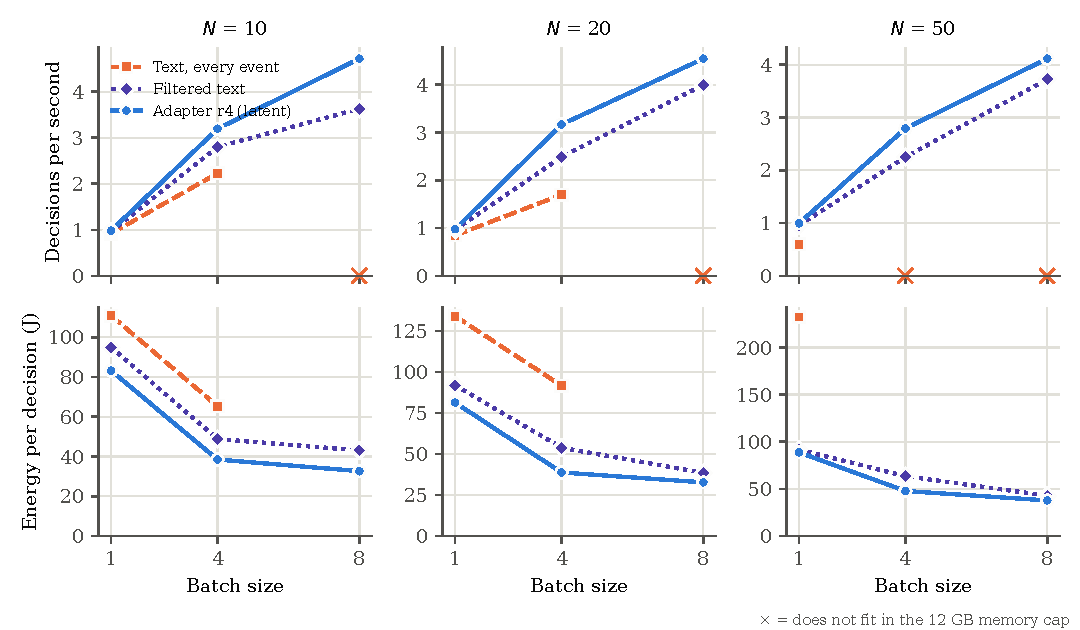
\includegraphics[width=\linewidth]{figures/fig_serving.pdf}
\caption{Throughput (top) and GPU energy per decision (bottom) when requests are batched, for 10, 20 and 50 events per prompt (final adapter, first training seed; medians). A cross marks a configuration that did not fit in the memory cap of the 12~GB card. Filtered text at batch eight is plotted from the batches that fit, which are its shortest prompts.}
\label{fig:serving}
\end{figure}

\subsection{RQ2: Accuracy}
\textbf{Against text that lists every event.} Default compact text falls from 0.97 balanced accuracy at one event to 0.48 to 0.56 at 10 to 50 events. Calibration recovers part of this (0.73 to 0.76) and is the fair comparison. The final adapter holds 0.81 to 0.84 at 5 to 50 events (Table~\ref{tab:accuracy}). Against calibrated text, the adapter was superior at 10 and 20 events (both $+0.10$, intervals excluding zero) and non-inferior at 5 and 50 events. At a single event, text was better (0.97 against 0.80), as expected from the cost analysis.

\begin{table}[t]
\caption{Balanced accuracy on class-balanced DS2 windows, and adapter minus calibrated text with 95\% patient-cluster intervals. Rule: the reference rule applied directly to the sender's outputs, 1 by construction and computed in microseconds; it is the ceiling of every channel and shows that the task itself does not need a language model (Section~\ref{sec:intro}). The adapter is superior at $N=10$ and 20 (interval above zero) and non-inferior at $N=5$ and 50 (lower limit above the margin of $-0.05$).}
\label{tab:accuracy}
\centering
\small
\begin{tabular}{rrrrrl}
\toprule
$N$ & Rule & Text & Text cal. & Adapter & Adapter $-$ cal. text [95\% CI] \\
\midrule
1 & 1.00 & 0.97 & 0.97 & 0.80 & --- \\
5 & 1.00 & 0.73 & 0.79 & 0.81 & $+0.03$ [$-0.04$, $+0.10$] \\
10 & 1.00 & 0.56 & 0.73 & 0.83 & $+0.10$ [$+0.03$, $+0.17$] \\
20 & 1.00 & 0.48 & 0.73 & 0.83 & $+0.10$ [$+0.01$, $+0.18$] \\
50 & 1.00 & 0.54 & 0.76 & 0.84 & $+0.08$ [$-0.02$, $+0.17$] \\
\bottomrule
\end{tabular}

\end{table}

\begin{figure}[t]
\centering
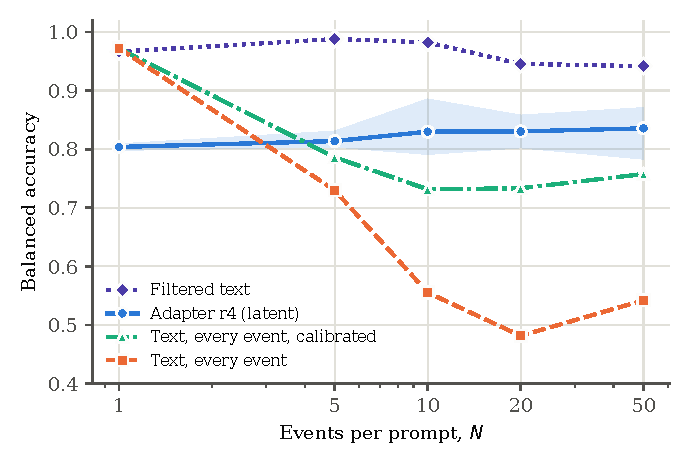
\includegraphics[width=0.85\linewidth]{figures/fig_accuracy.pdf}
\caption{Balanced accuracy against the number of events per prompt on the class-balanced test windows. The shaded band is the range of the three adapter seeds. Filtered text is the most accurate arm; text with every event listed degrades as events are added and calibration recovers only part of the loss.}
\label{fig:accuracy}
\end{figure}

\textbf{Why text with every event fails.} Two mechanisms account for most of the loss (Figure~\ref{fig:mechanisms}). Text misses urgent windows caused by a single high-confidence ventricular or fusion beat (a numeric threshold of 0.85 buried in a long list) far more often than windows caused by a run of abnormal beats. This is the clearest effect: text recalls 0.17 of such windows against 0.82 for the adapter. The position of the deciding beat points the way reported for long contexts \cite{liu2024lost,hsieh2024found}: text accuracy is lowest when that beat is in the middle third of the window (0.19, against 0.30 in the first and 0.38 in the last third). The evidence is weak. The middle group has 73 windows and its interval overlaps those of the other thirds (right panel of Figure~\ref{fig:mechanisms}), and the adapter shows a similar small dip (0.74 to 0.78 across positions). We report a position effect as suggested for text, not established, and not distinguishable from the adapter's.

\begin{figure}[t]
\centering
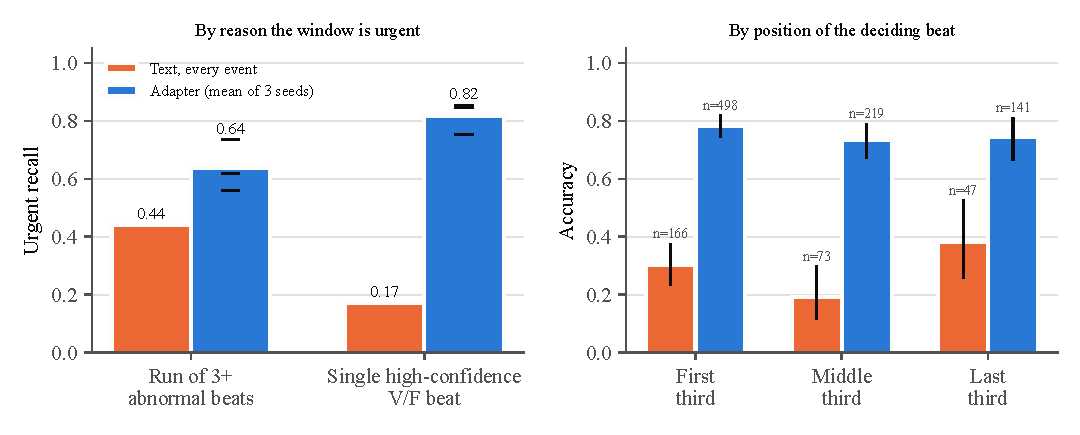
\includegraphics[width=0.65\linewidth]{figures/fig_mechanisms.pdf}
\caption{Urgent recall by the reason a window is urgent. Text with every event listed misses windows made urgent by a single high-confidence ventricular or fusion beat far more often than windows made urgent by a run; the adapter does not show this gap. Bars for the adapter are the mean of three seeds, with each seed's value marked. Right: accuracy on non-routine windows with $N \ge 10$ by the position of the window's most urgent beat; whiskers are 95\% Wilson intervals, and the adapter counts are windows times three seeds. This panel is exploratory (not in the analysis plan) and is computed by \texttt{scripts/position\_effect.py}.}
\label{fig:mechanisms}
\end{figure}

\textbf{False alarms.} The earlier adapter escalated about 11\% of routine windows, concentrated on windows with a normal beat of low classification confidence. The final adapter reduced the rate at every seed, by 44 to 80\% (about two thirds on average), to 3.6\% overall (0\% to 3.8\% at 50 events). Text raised none, because its error is the opposite one: it under-escalates urgent windows to priority. The adapter never called an urgent window routine in the 50-event confusion matrix.

\textbf{What the final adapter's gain comes from.} The final adapter differs from the earlier one in two ways: hard-negative routine windows in training, and three side inputs per event (heart rate, interval and run length). We retrained it without the side inputs, with three seeds and everything else identical (Table~\ref{tab:ablation}). The side inputs account for most of the improvement. Accuracy rose at every $N$ (by 0.03 to 0.05, with the interval excluding zero at 50 events) and false alarms fell from 8.6\% to 3.6\% in every seed. Hard negatives alone moved accuracy by about 0.01 and false alarms from 10.6\% to 8.6\%. The false-alarm reduction therefore comes mainly from giving the receiver the context to tell a low-confidence normal beat from a real event, not from the extra training examples.

\begin{table}[t]
\caption{Ablation of the final adapter (three seeds each): balanced accuracy, false alarms (FA) on routine windows, and the two contrasts with patient-cluster 95\% intervals. Hard negatives: hard-negative routine windows in training; side inputs: heart rate, interval and run length. The side-input contrast is clean (same windows and schedule); the hard-negative contrast is approximate, because the earlier adapter also used fewer training windows and a proportionally shorter schedule.}
\label{tab:ablation}
\centering
\footnotesize
\adjustbox{max width=\linewidth}{\begin{tabular}{lccccr}
\toprule
Recipe & $N$=5 & $N$=10 & $N$=20 & $N$=50 & FA \\
\midrule
r3 (neither) & 0.794 & 0.772 & 0.795 & 0.770 & 10.6\% \\
HN only & 0.788 & 0.786 & 0.802 & 0.781 & 8.6\% \\
r4 (HN + SI) & 0.814 & 0.830 & 0.830 & 0.836 & 3.6\% \\
SI: r4 $-$ HN only & $+0.03$ [$-0.02$, $+0.06$] & $+0.04$ [$-0.01$, $+0.11$] & $+0.03$ [$-0.01$, $+0.07$] & $+0.05$ [$+0.01$, $+0.11$] &  \\
HN: HN only $-$ r3 & $-0.01$ [$-0.04$, $+0.03$] & $+0.01$ [$-0.02$, $+0.05$] & $+0.01$ [$-0.04$, $+0.05$] & $+0.01$ [$-0.03$, $+0.05$] &  \\
\bottomrule
\end{tabular}
}
\end{table}

\textbf{Against text that lists only abnormal events.} A-filtered was more accurate than the adapter at every $N$ (Table~\ref{tab:filtered}), raised no false alarms, and for a single request matched it in time to first token and to decision within 1.5\%. Its cost depends on content: each listed abnormal beat adds about 68 tokens, so at 50 events its prompt is longer than the adapter's in half of the windows. The decision rule fixed in the analysis plan anticipated a filtered prompt that was cheaper but less accurate; applied literally it returned ``advantage holds'' because the filtered prompt turned out to be longer. We do not read it that way. Against filtered text, on this task, the latent interface has no accuracy advantage and no latency advantage for a single request.

\begin{table}[t]
\caption{Adapter against filtered text (default decoding) with patient-cluster intervals, and median prompt tokens (adapter / filtered).}
\label{tab:filtered}
\centering
\small
\begin{tabular}{rrrrr}
\toprule
$N$ & Adapter r4 & Filtered & Difference [95\% CI] & Tokens \\
\midrule
1 & 0.804 & 0.966 & --- & 516 / 679 \\
5 & 0.814 & 0.988 & $-0.17$ [$-0.22$, $-0.13$] & 532 / 679 \\
10 & 0.830 & 0.982 & $-0.15$ [$-0.19$, $-0.11$] & 553 / 682 \\
20 & 0.830 & 0.945 & $-0.12$ [$-0.16$, $-0.07$] & 593 / 683 \\
50 & 0.836 & 0.942 & $-0.11$ [$-0.17$, $-0.05$] & 713 / 750 \\
\bottomrule
\end{tabular}

\end{table}

\textbf{Against the annotations.} Scored against the database annotations instead of the sender's own rule, with a window counted as abnormal if any of its beats is annotated as not normal, the reference rule has sensitivity of 0.94 to 0.96 and specificity of only 0.46 to 0.64 across window sizes. The clinical ceiling is therefore set by perception and not by the interface: the final adapter tracked the reference (sensitivity 0.90 to 0.96 at 5 to 50 events), while default compact text missed more abnormal windows (0.77 to 0.79 at 10 to 50 events).

\textbf{Second sender.} The replication with a convolutional sender (validation accuracy 0.955 against a gate of 0.85) reproduced the pattern (Table~\ref{tab:second}). Text with every event listed fell as events were added while the adapter stayed at 0.77 to 0.82; the adapter was superior to calibrated text at 10 events and non-inferior at 20 and 50, but not at 5; false alarms were 1.3 to 2.1\%. A-filtered was again the most accurate arm except at 50 events, where it fell to 0.80 and the difference was inconclusive ($-0.01$ [$-0.09$, $+0.08$]). An exploratory look at those windows (40 per sender, so indicative only) suggests that this sender's urgent windows carry sparser, more borderline evidence, often one urgent beat among about 13 listed abnormal beats with a deciding confidence just above 0.85. Filtered text depends on how the sender's evidence is distributed, whereas the adapter did not change much.

\begin{table}[t]
\caption{Second sender (ResNet1D-RR): balanced accuracy on its own DS2 windows and adapter minus calibrated text (non-inferiority margin $-0.05$).}
\label{tab:second}
\centering
\footnotesize
\begin{tabular}{rrrrl}
\toprule
$N$ & Adapter & Text cal. & Filtered & Adapter $-$ cal. text [95\% CI] \\
\midrule
5 & 0.770 & 0.787 & 0.959 & $-0.02$ [$-0.11$, $+0.08$] \\
10 & 0.823 & 0.732 & 0.929 & $+0.09$ [$+0.02$, $+0.16$] \\
20 & 0.780 & 0.733 & 0.907 & $+0.05$ [$-0.03$, $+0.13$] \\
50 & 0.794 & 0.733 & 0.808 & $+0.06$ [$-0.02$, $+0.14$] \\
\bottomrule
\end{tabular}

\end{table}

\textbf{External confirmatory test.} The frozen system was evaluated once on a second database; the result is reported in Section~\ref{sec:incart}.

\subsection{RQ3: What Can Be Recovered}
\textbf{Single events.} Decoders trained on the training records and applied to the test records recovered the predicted beat label (accuracy 99.5\%) and tier (95\%; balanced accuracy 0.88) from the virtual tokens of the single-event adapters as well as from the 32-dimensional input, so the adapter loses nothing the vector holds.

\textbf{Every position.} For slots 0, 9, 19 and 49 of a 50-event window, label, tier and urgency decoded at the level of the input vector. Decoders are slot-specific: a decoder trained on slot 0 applied at slot 49 fell to 0.64 to 0.91, so an auditor needs a position-aware decoder.

\textbf{What the vector never carried.} The 32-dimensional context vector does not contain heart rate, interval or run length ($R^2$ about 0.3), so the earlier adapter could not carry them either. With the side inputs of the final adapter they are recoverable from the tokens (Table~\ref{tab:recover}). The decoder specified in advance was a small multilayer perceptron, and with it heart rate ($R^2$ 0.59 to 0.78) and interval (0.65 to 0.77) fall well short of the input (0.98 and 0.95), while the presence of a run of three abnormal beats is recovered at 0.93 to 0.98 balanced accuracy (0.53 to 0.61 for the earlier adapter, near chance). A linear decoder, fitted in the same analysis, recovers much more of the numeric fields from the same tokens (heart rate 0.95 to 0.97, interval 0.92 to 0.96). The multilayer decoder therefore understates what the tokens hold, and the information is held in a nearly linear form. We report both: the figure from the decoder specified in advance is the conservative one, and the linear figures are the better estimate of what an auditor could recover. On the second sender, heart rate and interval are recovered from every token slot at $R^2$ 0.89 to 0.94 with the decoder specified in advance. Signal quality is not carried by either sender.

\begin{table}[t]
\caption{Recoverability of each event's fields from its virtual tokens (final adapter, main sender), decoders trained on the training records and applied to the test records. Token columns give the range over slots 0 and 49 and three seeds. The multilayer perceptron was the decoder specified in advance; the linear decoder is reported for comparison.}
\label{tab:recover}
\centering
\footnotesize
\adjustbox{max width=\linewidth}{\begin{tabular}{lrrrr}
\toprule
Field & Input, MLP & Tokens, MLP & Input, linear & Tokens, linear \\
\midrule
Beat label (bal. acc.) & 0.99 & 0.95--0.98 & 0.99 & 0.99--1.00 \\
Tier (bal. acc.) & 0.95 & 0.92--0.95 & 0.91 & 0.90--0.94 \\
Urgency flag (bal. acc.) & 0.98 & 0.97--0.98 & 0.94 & 0.94--0.95 \\
Heart rate ($R^2$) & 0.98 & 0.59--0.78 & 1.00 & 0.95--0.97 \\
RR interval ($R^2$) & 0.95 & 0.65--0.77 & 0.98 & 0.92--0.96 \\
Run $\geq 3$ (bal. acc.) & 0.98 & 0.93--0.98 & 0.95 & 1.00--1.00 \\
\bottomrule
\end{tabular}
}
\end{table}

\textbf{Carried and used.} The ablation shows both directions. Without the side inputs, heart rate, interval and run length are not recoverable from the tokens at all ($R^2$ at most 0.09; run $\geq 3$ at 0.52 to 0.59, near chance); with them they are, and the receiver uses them, since they account for most of the accuracy gain and the false-alarm reduction (Table~\ref{tab:ablation}). Use is partial, however: urgent recall on windows made urgent by a run of three or more abnormal beats rose only from 0.61 to 0.64 when run length entered the tokens, against 0.44 for text.

\textbf{Pre-generation check.} For the single-event adapters, scores computed from the context vector alone flag inputs before generation: a tier decoder predicts the adapter's wrong answers (AUROC 0.89 to 0.97), and a Mahalanobis distance flags noise and powerline interference (0.99). This gives an inspection that does not need to read the tokens.

\textbf{Compression.} We retrained the adapter with one, two and eight virtual tokens per event in place of four (Table~\ref{tab:sweep}, Figure~\ref{fig:sweep}). A first sweep with one seed per setting suggested that a single token might suffice, so one and two tokens were repeated with three seeds each, under a rule fixed before training: a setting is free of accuracy cost only if it is non-inferior to four tokens (margin $-0.05$) at every $N$. Neither passed. With one token, one run in three failed to learn the task (0.49 to 0.55 at 5 to 50 events) while the other two matched four tokens, so the three-seed mean was 0.09 to 0.11 lower. With two tokens accuracy was within about 0.01 of four tokens at 5 to 20 events and 0.04 lower at 50, non-inferior only at 20 events, and false alarms were higher in every run (8.6\% on average against 3.6\%). Eight tokens, a single run, was no better than four. Each event's label, heart rate and run status remained recoverable from a single token, including from the one-token run that failed the task (label 0.96 to 0.99, heart-rate $R^2$ about 0.9 with the decoder specified in advance). Compression below four tokens per event therefore preserved what the tokens carry but made the receiver's use of it unreliable, and four tokens was the smallest setting at which every run was reliable. The saving would be modest in any case, because the scaffold dominates: at 50 events, 563 tokens at one token per event against 713 at four.

\begin{table}[t]
\caption{Virtual tokens per event: three seeds for $k$ = 1, 2 and 4 (means), one run for $k$ = 8. Tokens: prompt length at 50 events. $k-4$: difference from $k$ = 4 at the least favourable $N$ (50 in both cases), with its patient-cluster 95\% interval; NI: number of $N$ (of 5, 10, 20, 50) at which $k$ is non-inferior (margin $-0.05$). FA: false alarms on routine windows (seed ranges in the text). Label and HR $R^2$: recoverability from slot 0 with the decoder specified in advance (multilayer perceptron); the negative $R^2$ at $k$ = 8 is likely a decoder limit (32 principal components of a 20,480-dimensional slot).}
\label{tab:sweep}
\centering
\footnotesize
\adjustbox{max width=\linewidth}{\begin{tabular}{rrclcrrr}
\toprule
$k$ & Tokens & Bal. acc., $N$ = 5/10/20/50 & $k-4$ [95\% CI] & NI & FA & Label & HR $R^2$ \\
\midrule
1 & 563 & 0.70 / 0.72 / 0.75 / 0.73 & $-0.11$ [$-0.16$, $-0.06$] & 0/4 & 6.3\% & 0.97 & $0.87$ \\
2 & 613 & 0.80 / 0.82 / 0.83 / 0.80 & $-0.04$ [$-0.13$, $+0.03$] & 1/4 & 8.6\% & 0.95 & $0.81$ \\
4 & 713 & 0.81 / 0.83 / 0.83 / 0.84 & ref. & -- & 3.6\% & 0.96 & $0.71$ \\
8 & 913 & 0.77 / 0.80 / 0.78 / 0.80 & 1 run & -- & 6.1\% & 0.95 & $-0.62$ \\
\bottomrule
\end{tabular}
}
\end{table}

\begin{figure}[t]
\centering
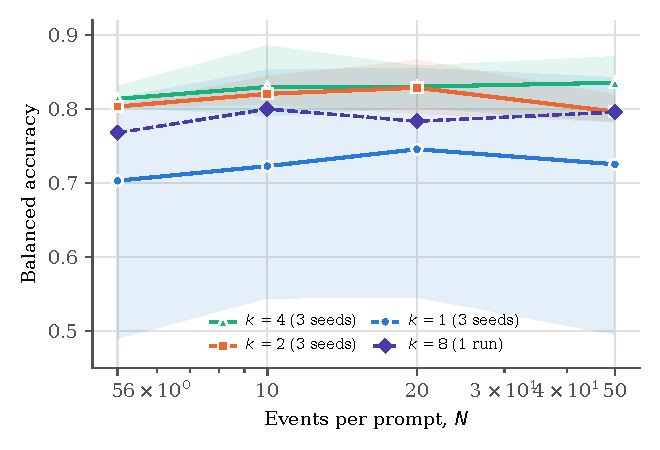
\includegraphics[width=0.7\linewidth]{figures/fig_sweep.pdf}
\caption{Balanced accuracy against the number of events for $k$ = 1, 2 and 4 virtual tokens per event (lines: mean of three seeds; bands: seed range) and $k$ = 8 (one run). The wide band at $k$ = 1 is one failed run.}
\label{fig:sweep}
\end{figure}

\subsection{External Confirmatory Test on INCART}
\label{sec:incart}
The DS2 test set informed several design iterations, so its results cannot confirm the final system. The confirmatory test is therefore a single run of the frozen system on a database that played no part in any decision. The St Petersburg INCART database has 75 half-hour recordings from 32 patients; after conversion to the same beat format (lead II, resampled from 257 to 360~Hz) it yields 175,777 accepted beats: 153,594 normal, 20,006 ventricular, 1,958 supraventricular and 219 fusion beats. A further 91 beats whose window fell outside the recording and 51 with an unmapped annotation symbol were excluded. The test set has 1,240 windows with every stratified cell filled (Table~\ref{tab:incartwindows}), and its hash was committed before any model output existed.

\begin{table}[t]
\caption{INCART test windows by number of events per prompt $N$ and reference tier. All stratified cells reached their quota.}
\label{tab:incartwindows}
\centering
\footnotesize
\adjustbox{max width=\linewidth}{\begin{tabular}{rrrrrrr}
\toprule
$N$ & Routine & Priority & Urgent & Stratified & Natural prevalence & Total \\
\midrule
1 & 60 & 60 & 60 & 180 & --- & 180 \\
5 & 60 & 60 & 60 & 180 & 100 & 280 \\
10 & 60 & 60 & 60 & 180 & 100 & 280 \\
20 & 60 & 60 & 60 & 180 & 100 & 280 \\
50 & 40 & 40 & 40 & 120 & 100 & 220 \\
All &  &  &  & 840 & 400 & 1240 \\
\bottomrule
\end{tabular}
}
\end{table}

The system under test was fixed in a manifest of file hashes before the run: the three final adapters (not retrained), the perception agent, the prompt and decoding code, and the calibration biases chosen on the DS1 validation windows and not re-tuned. Text arms were generated by stopping at the tier token, as decided after that choice was shown on DS2 to change no tier. The four hypotheses were tested in a fixed sequence at $\alpha = 0.05$, stopping at the first failure, with patient-cluster bootstrap intervals (20,000 resamples): \textbf{H1}, the adapter (three-seed mean) is non-inferior to calibrated compact text at $N$ = 10, 20 and 50 (margin $-0.05$, all three required); \textbf{H2}, it is superior at $N$ = 10 and 20; \textbf{H3}, it is non-inferior to calibrated filtered text at $N$ = 10, 20 and 50; \textbf{H4}, its median time to first token is lower than that of compact text at $N$ = 10, 20 and 50. Hypotheses after the first failure are reported descriptively as not tested in sequence.

\begin{table}[t]
\caption{Hypotheses on INCART, fixed in advance. Estimates are adapter minus calibrated text (H1, H2), adapter minus calibrated filtered text (H3), or the median relative difference in time to first token (H4), with 95\% intervals. H4 was not tested in sequence because H3 failed. $^\dagger$The time-to-first-token value at 50 events is the technical re-measurement under the memory cap (see text); the original value ($-0.97$) was distorted by memory paging.}
\label{tab:incarthyp}
\centering
\footnotesize
\adjustbox{max width=\linewidth}{\begin{tabular}{llrrll}
\toprule
Hypothesis & $N$ & Estimate & 95\% CI & Result & Status \\
\midrule
H1: non-inferior to calibrated text & 10 & $+0.08$ & [$+0.03$, $+0.15$] & pass & confirmed \\
 & 20 & $+0.09$ & [$+0.04$, $+0.15$] & pass &  \\
 & 50 & $+0.05$ & [$-0.04$, $+0.13$] & pass &  \\
H2: superior to calibrated text & 10 & $+0.08$ & [$+0.03$, $+0.15$] & pass & confirmed \\
 & 20 & $+0.09$ & [$+0.04$, $+0.15$] & pass &  \\
H3: non-inferior to calibrated filtered text & 10 & $-0.11$ & [$-0.17$, $-0.05$] & fail & not confirmed \\
 & 20 & $-0.11$ & [$-0.16$, $-0.06$] & fail &  \\
 & 50 & $-0.07$ & [$-0.15$, $-0.00$] & fail &  \\
H4: faster first token than text & 10 & $-0.27$ & [$-0.28$, $-0.26$] & pass & not tested in sequence \\
 & 20 & $-0.51$ & [$-0.52$, $-0.49$] & pass &  \\
 & 50$^\dagger$ & $-0.77$ & [$-0.78$, $-0.77$] & pass &  \\
\bottomrule
\end{tabular}
}
\end{table}

\begin{table}[t]
\caption{Balanced accuracy on INCART by number of events per prompt (adapter: mean of three seeds). Rule: the reference rule on the sender's outputs, 1 by construction.}
\label{tab:incartacc}
\centering
\footnotesize
\adjustbox{max width=\linewidth}{\begin{tabular}{rrrrrrr}
\toprule
$N$ & Rule & Adapter & Text & Text cal. & Filtered & Filtered cal. \\
\midrule
1 & 1.000 & 0.746 & 0.983 & 0.978 & 0.972 & 0.972 \\
5 & 1.000 & 0.789 & 0.722 & 0.806 & 0.939 & 0.933 \\
10 & 1.000 & 0.815 & 0.583 & 0.733 & 0.939 & 0.922 \\
20 & 1.000 & 0.822 & 0.517 & 0.728 & 0.933 & 0.928 \\
50 & 1.000 & 0.822 & 0.533 & 0.775 & 0.892 & 0.892 \\
\bottomrule
\end{tabular}
}
\end{table}

\begin{table}[t]
\caption{Routine windows escalated to priority or urgent on INCART.}
\label{tab:incartfa}
\centering
\footnotesize
\begin{tabular}{lrr}
\toprule
Arm & All routine windows & Natural prevalence \\
\midrule
Adapter, seed 101 & 0.2\% & 0.0\% \\
Adapter, seed 202 & 3.3\% & 2.8\% \\
Adapter, seed 303 & 1.1\% & 1.1\% \\
Text, calibrated & 0.0\% & 0.0\% \\
Filtered, calibrated & 0.0\% & 0.0\% \\
\bottomrule
\end{tabular}

\end{table}

Both hypotheses on accuracy against calibrated compact text were confirmed (Table~\ref{tab:incarthyp}). The adapter's three-seed mean was non-inferior at 10, 20 and 50 events (H1) and superior at 10 and 20 events (H2): the differences were $+0.08$ [$+0.03$, $+0.15$] at 10 events and $+0.09$ [$+0.04$, $+0.15$] at 20 events, with patient-cluster intervals, and the margin at 50 events was cleared narrowly ($+0.05$ [$-0.04$, $+0.13$] against a margin of $-0.05$). These estimates are close to those on the MIT-BIH test set ($+0.10$ at both 10 and 20 events), on a different database, a different lead resampled from 257 to 360~Hz, and different patients. The result for the filtered text was the opposite, and H3 was not confirmed. Filtered text was the most accurate arm at every number of events above one (0.89 to 0.94 against 0.82 for the adapter at 10 to 50 events, Table~\ref{tab:incartacc}), and the adapter was inferior to it at every tested size: $-0.11$ at 10 and 20 events and $-0.07$ at 50 events, with every interval excluding zero (at 50 events only just, [$-0.15$, $-0.004$]). Following the rule fixed in advance, H4 is therefore reported as not tested in sequence. It is described below.

\textbf{Accuracy by window size.} The pattern matches MIT-BIH. At a single event text is more accurate than the adapter (0.98 against 0.75). Text that lists every event degrades as events are added, from 0.72 at 5 events to 0.53 at 50 events under default decoding, and calibration recovers part of the loss (0.73 to 0.81). The adapter stays between 0.79 and 0.82 at 5 to 50 events, with a seed range of 0.79 to 0.84 at 10 events (Table~\ref{tab:incartacc}).

\textbf{False alarms and parsing.} Every arm produced a valid answer on every window (parse rate 100\%). Text and filtered text raised no false alarms. The adapter escalated 0.2\%, 3.3\% and 1.1\% of routine windows for the three seeds, the same range as or lower than the 2.7 to 4.8\% of the three seeds on MIT-BIH. In 11 to 16\% of windows the adapter's free-text fields reached the fixed length cap; the field-cap rate is undefined for the text arms, which were stopped at the tier token.

\textbf{Time to first token (descriptive).} The adapter's prompt-processing time stayed near 180 to 200~ms at every number of events, as on MIT-BIH, while that of compact text rose with the prompt. The median relative difference was $-27\%$ at 10 events and $-51\%$ at 20 events, within a few points of the MIT-BIH values ($-24\%$ and $-50\%$), and each interval excluded zero. At 50 events the confirmatory run's timing of compact text was not usable: it took a median 6.9~s, with a range of 3.3 to 15.3~s across the 21 windows, against 0.85~s for a prompt of the same length on MIT-BIH, which is the signature of memory paging on the 12~GB card, a condition controlled in the serving measurements with a memory cap (Section~\ref{sec:protocol}) but not in this timing routine. We therefore re-measured that step alone, documented before the measurement as a technical change to the protocol: the same frozen routine, on the same 21 windows, with the memory cap applied and cached memory released before each timed call, outside the timer. Compact text then took a median 859~ms (maximum 881~ms), the adapter 194~ms and filtered text 195~ms, so the adapter was $-77\%$ [$-78\%$, $-77\%$] faster than compact text (MIT-BIH: $-78\%$) and not different from filtered text ($-2\%$ [$-15\%$, $+3\%$]). The original measurement is kept on record. H4 remains not tested in sequence, and these figures are descriptive.

\textbf{What the confirmatory test establishes.} On a second database that played no part in any decision, the accuracy advantage of the adapter over calibrated compact text replicated at 10 and 20 events, and the advantage of a sender-side filter over the adapter replicated at every number of events. The test does not show that the adapter beats the best text interface, and it does not test the unknown-question case, for which no experiment here has a fixed answer. Perception accuracy on INCART is not an endpoint and is not reported here.

\section{Discussion}
\label{sec:discussion}

\subsection{Choosing a Communication Interface}
The three research questions give three answers, and they do not point to the same arm. Table~\ref{tab:selection} sets the arms side by side on the criteria a system designer would use. Reading across it, no interface dominates: the filter wins on accuracy and readability, the latent channel on predictability of cost under load, and listing every event on nothing except simplicity at small $N$.

\begin{table}[t]
\caption{Interfaces compared on the criteria that decide the choice, from the measurements in Section~\ref{sec:results}. ``Content-dependent'' means that the cost varies with how many abnormal events a window contains.}
\label{tab:selection}
\centering
\footnotesize
\begin{tabular}{p{2.3cm}p{3.1cm}p{3.1cm}p{3.1cm}}
\toprule
Criterion & Text, every event & Filtered text (say less) & Adapter (latent) \\
\midrule
Accuracy ($N\!\ge\!10$) & Lowest, even calibrated & Highest & Between; above calibrated text at $N$ = 10, 20 \\
Prompt length & Grows with $N$ & Content-dependent & Depends only on $N$ \\
Single-request latency & Grows with $N$ & Equal to adapter within about 5\% & Flat in $N$ \\
Batched throughput and energy & Does not fit at batch 8 or at $N=50$ & Between; fits only some batches & Highest; fits every configuration \\
Memory planning & Impossible at large $N$ & Content-dependent & Fixed per event \\
False alarms & None & None & 1 to 4\% of routine windows \\
Auditability & Readable & Readable; normal events dropped & Needs a position-aware decoder \\
\bottomrule
\end{tabular}
\end{table}

From the table we draw a selection rule for the task studied, with one part stated as a hypothesis.
\begin{itemize}
\item \textbf{The receiver's question is fixed and known when the sender writes its message:} filter on the sender side and send text. The filter was the most accurate arm at almost every $N$ on both senders, raised no false alarms, matched the adapter for a single request, and can be read by a person without any decoder.
\item \textbf{Many events must be communicated at a predictable cost, or requests are batched on constrained hardware:} use the latent channel. Its length depends only on $N$, so memory and batch size can be planned in advance, and in the batched measurements it delivered 10 to 30\% more decisions per second at 12 to 28\% less energy per decision than filtered text.
\item \textbf{The question is not known when the sender encodes} (hypothesis, not tested here): a filter cannot discard what it cannot rank, whereas the latent channel carries information about every event. Our task has one question, so the experiment cannot show that the extra information would be used by a different one. A study that varies the question over fixed virtual tokens is the direct test, and we leave it to future work.
\end{itemize}
Against text that lists every event, the adapter wins on cost and, at moderate window sizes, on accuracy, but that is a comparison with a prompt no careful engineer would send.

This rule is a communication policy of the kind that recent edge-intelligence work formalises, in which the system decides what to send and in what form according to conditions \cite{aei2026survey,dai2026tokenkv}. Existing policies choose between text and a transformer's cache. Our results add a third option for senders that are not transformers and show that, for them, the choice turns on the shape of the workload and the serving regime more than on accuracy.

\subsection{Why the Filter Wins on Accuracy and the Adapter Wins Under Load}
The two results have different causes. The filter is accurate because it uses the sender's own labels to remove exactly the events that cannot change the answer, leaving a short list the receiver can reason over; its accuracy therefore depends on how the sender's evidence is distributed, as the second sender shows, where filtered text fell at 50 events when urgent windows rested on a single borderline beat among many. The adapter is less accurate, and we offer two plausible reasons that this study does not separate: the receiver has to learn from a small training set to read tokens that were never part of its vocabulary, and the linear map from a classification-trained vector carries less than the sender's text fields do (the side inputs of the final recipe were added to close that second gap; the ablation shows they drive the final recipe's gain, and the run-length result shows the gap only partly closed). It wins under load for a structural reason: the filter's length is a function of content, so batches of long prompts do not fit, whereas the adapter's length is a function of $N$ alone. The first is a property of the sender's output and the second a property of the interface, and a designer who knows the workload can read off which regime applies.

\subsection{What the Result Means for Auditability}
The standing objection to a latent channel is that no one can read it. We find that much can be read back by training decoders on the tokens: label, tier and abnormal-run status at the level of the input, and heart rate and interval nearly so with a linear decoder, at every slot tested. What an auditor needs is a position-aware decoder per slot, and what the channel does not carry (signal quality) is identified by the same method. But recoverable is not the same as used. The compression study shows this most clearly: at one virtual token per event every field remained recoverable, including from a run that failed the task, so a recoverability audit can certify what the channel carries but not that the receiver relies on it. The run-length experiment shows a field that reaches the language model without being used reliably, and a pre-generation score computed from the context vector gives an inspection that does not depend on the tokens at all. Zhang and Emu show, for latent channels between language models, that equal end-task accuracy can arise from opposite mechanisms and that a message must be replaced to know whether it matters \cite{zhang2026causalaudit}. The same discipline applies here, and the null and shuffle controls registered in the analysis plan are the receiver-side half of the measurement. \todo{State their results here if they are part of the final analysis; otherwise list as future work.}

\subsection{Limitations}
\begin{itemize}
\item \textbf{The task is a fixed rule.} The reference answer is a three-line rule over the perception outputs, so a language model is not needed for the answer. The study measures a channel, not reasoning, and says so. It does not show that the language model contributes judgement.
\item \textbf{One receiving model.} All results use Gemma~4 E4B in 4-bit quantisation. A second receiver, of a different family, is future work, and the adapter is specific to one embedding space.
\item \textbf{One database for tuning, one external test.} The primary test set informed several design iterations. Each was logged before the data it affected, but the set is no longer untouched. The external confirmatory test on INCART was fixed for this reason \todo{update with the result}.
\item \textbf{Training variance.} Outcomes vary between training seeds (validation balanced accuracy 0.72 to 0.82 for r4, and one failed run at one token per event), so every adapter result is reported over three seeds; the eight-token setting is a single run.
\item \textbf{Perception quality.} Specificity of the encoder's rule against the annotations is 0.46 to 0.52, and fusion beats are almost never detected. The ceiling on usefulness is set upstream of the interface.
\item \textbf{Zero-shot text baseline.} The adapter was trained on the task while the text arms are zero-shot under a frozen-model constraint. A trained text baseline would narrow the accuracy gap and was not run.
\item \textbf{Fairness of calibration.} Calibration chose a single bias on the routine score. A richer calibration could further improve text with every event listed.
\item \textbf{Hardware and software.} Timing was measured on one consumer GPU through a general-purpose framework, because production engines do not accept continuous embeddings; only relative results are meaningful. Network transfer between agents was not measured, because both agents ran on one machine.
\item \textbf{Clinical use.} The system is a research prototype. No clinician rated its outputs, and nothing here supports clinical deployment.
\end{itemize}

\subsection{Implications for System Design}
Three practical points follow. First, the value of a latent channel is a property of the workload and not of the channel: report cost against the number of events and under batching, and include a filtered text baseline, or the comparison says little. Second, a fixed per-event footprint changes how a system is provisioned even where accuracy is equal, because batch size no longer depends on what the sender has to say. Third, inspectability can be measured and not merely asserted: train decoders on the message and report what they recover, per slot and per field.

\section{Conclusion}
\label{sec:conclusion}
For a perception agent that is not a transformer, there is a choice of how to talk to a frozen language model, and it is not settled by accuracy alone. A sender-side filter is the more accurate and more readable interface when the receiver's question is known in advance. A four-token-per-event linear adapter gives a latent channel whose cost is fixed per event, which is more accurate than calibrated compact text at moderate window sizes and, under batched serving on constrained hardware, serves more decisions per second at lower energy than the filter, while the content of each event remains recoverable from its tokens. We give a rule for choosing between them and release the pre-registration log, the harness and the analysis, so that the comparison can be repeated for other senders, receivers and tasks.


\bibliographystyle{elsarticle-num}
\bibliography{refs}

\end{document}
